\documentclass[a4paper]{article}

\usepackage[utf8]{inputenc}

\usepackage{graphicx,float}
\graphicspath{ {./resources/} }
\newcommand{\mockupheight}{0.4\textheight}

\usepackage{tabularx,enumitem}
\usepackage{booktabs}
\newcommand{\tabitem}{~~\llap{\textbullet}~~}

\setlength{\parindent}{0pt}

\usepackage{listings}
\lstset{
basicstyle=\ttfamily,
breaklines = true,
tabsize=2
}

\usepackage[hidelinks]{hyperref}

%https://github.com/Angtrim/alloy-latex-highlighting
\usepackage[dvipsnames]{xcolor}
\usepackage{alloy}

\begin{document}

%----------------------------------------------------------------------------------------
%	TITLE PAGE
%----------------------------------------------------------------------------------------

\begin{titlepage}
	\newcommand{\HRule}{\rule{\linewidth}{0.5mm}}
	
	\center
	
	%------------------------------------------------
	%	Headings
	%------------------------------------------------
	
	\textsc{\LARGE Politecnico di Milano}\\[1.5cm]
	
	\textsc{\Large Computer Science and Engineering}\\[0.5cm]
	
	\textsc{\large Software Engineering 2}\\[0.5cm]
	
	%------------------------------------------------
	%	Title
	%------------------------------------------------
	
	\HRule\\[0.4cm]
	
	{\huge\bfseries SafeStreets\medskip\\
	\normalsize Requirement Analysis and Specification Document}\\[0.4cm]
	
	\HRule\\[1.5cm]
	
	%------------------------------------------------
	%	Author(s)
	%------------------------------------------------
	
	\begin{minipage}{0.4\textwidth}
		\begin{flushleft}
			\large
			\textit{Authors}\\
			\textsc{Simone Braga}\\
			\textsc{Juan Calderon}\\
			\textsc{Marzia Favaro}
		\end{flushleft}
	\end{minipage}
	~
	\begin{minipage}{0.4\textwidth}
		\begin{flushright}
			\large
			\textit{Professor}\\
			\textsc{Elisabetta Di Nitto}\linebreak\linebreak
		\end{flushright}
	\end{minipage}
	
	%------------------------------------------------
	%	Logo
	%------------------------------------------------
	
	\vfill\vfill\vfill
	
	\begin{figure}[H]
	\centering
	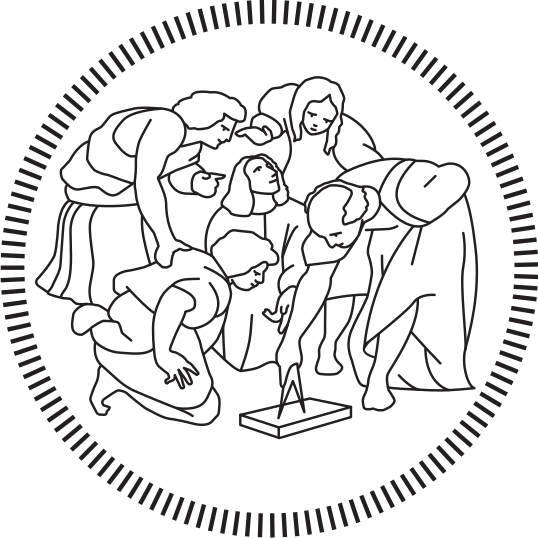
\includegraphics[width=0.5\textwidth]{polimi_logo}
	\end{figure}
	
	%------------------------------------------------
	%	Date
	%------------------------------------------------
	
	\vfill\vfill\vfill
	
	{\large\today\\ Version 1.1}
		%----------------------------------------------------------------------------------------
	
	\vfill
	
\end{titlepage}

%----------------------------------------------------------------------------------------

\newpage
\pagenumbering{roman}

\tableofcontents

\newpage
\pagenumbering{arabic}

\section{INTRODUCTION}\label{introduction}

\subsection{Purpose}

\textbf{SafeStreets} is a crowd-sourced application that intends to
provide users with the possibility to notify authorities when traffic
violations occur. The main target of the application are violations that
can be easily captured by a camera (like, for instance, parking
violations). SafeStreets intends also to provide users with the
possibility to mine the stored information with different levels of
visibility. Moreover, the application must cross the collected data with
information coming from the municipality to provide suggestions on
possible interventions to decrease the incidence of violations and
accidents. In the end, the application must forward data about
violations to generate traffic tickets, and must allow authorities to
get statistics on issued tickets.
\medskip\\
These requirements are exploited by developing several services:
\begin{itemize}
\item
  \textbf{SafeReports} allows common users to send violation reports.
\item
  \textbf{SafeAnalytics} allows common users and authorities to mine
  stored information.
\item
  \textbf{SafeTickets} allows authorities to get statistics on issued
  tickets.
\item
  \textbf{SafeSuggestions} allows municipality users to get suggestions
  on possible interventions.
\end{itemize}

\subsubsection{Goals}

The purpose of the software is captured by the following goals:
\begin{itemize}
\item
  \textbf{G1} SafeReports must allow common users to send violation
  reports.
\item
  \textbf{G2} SafeAnalytics must allow common users to get anonymous
  data on violations.
\item
  \textbf{G3} SafeAnalytics must allow authorities to access to all the
  data without restrictions.
\item
  \textbf{G4} SafeSuggestions must allow municipality users to get
  suggestions on possible interventions.
\item
  \textbf{G5} SafeStreets must generate traffic tickets forwarding
  reliable data to MTS.
\item
  \textbf{G6} SafeTickets must allow authorities to get statistics on
  issued tickets.
\end{itemize}

\subsection{Scope}

SafeStreets must interface with different types of users and information
sources. In this context, it is very important to identify the placement
of SafeStreets and its services with the entities of the scenario. To do
so, we will refer to the following picture. Afterward, every link
between SafeStreets and the entities will be deeply analyzed to
exhaustively describe the shared phenomena of the scenario.

\begin{figure}[H]
\centering
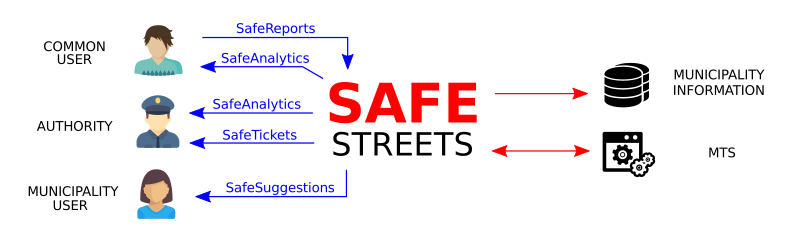
\includegraphics[width=\textwidth]{relationship_diagram}
\caption{Relationship diagram}
\end{figure}

Two types of interactions can be defined:
\begin{itemize}
\item
  \textbf{Interactions through services} (blue arrows in the diagram)
\item
  \textbf{Interactions with resources} (red arrows in the diagram)
\end{itemize}

The main difference between the interactions is the role of SafeStreets.
In the interactions through services, SafeStreets has a
passive role, in the sense that the activation of the interaction is
triggered by a request coming from the user through one of the offered
services. In the interactions with resources, SafeStreets has an active
role, in the sense that the activation of the interaction is
automatically triggered by SafeStreets application to exploit back-end
processes.
\medskip\\
Services are exploited differently depending on the type of user that is
enjoying the application. The type of the user is determined in the
registration phase, which is different depending on this choice.
Everyone can sign up as a common user. Instead, to sign up as an
authority or municipality user, it is necessary to provide a unique
disposable code, which assignment is not part of the application
(SafeStreets must take care only of the verification of the provided
code). The code is assigned only to users whose role declaration has
been manually verified by a human operator. For this reason, the
verification of authorities and municipality users is not considered in
the registration phase.

\subsubsection{SafeReports}

SafeReports is the core of the application. It provides common users
with the possibility to send a notification about a violation. To do so,
they are asked to take a picture of the vehicle involved in the
violation. Then the photo is checked and matched with some data captured
at the moment (position, date and time). The user is asked to review and
confirm the violation report that, in case of confirmation, is sent to
SafeStreets, which stores it to offer several other services.

\subsubsection{SafeAnalytics}

SafeAnalytics provides the possibility to mine SafeStreets data to get
information about violations. This service is offered to common users
and authorities, that can access data with different restriction levels.
Common users have access to anonymous data concerning a selected zone.
Authorities, instead, have access to unrestricted information on all the
stored data.

\subsubsection{SafeTickets}

SafeStreets uses Municipality Tickets Service (MTS) to generate traffic
tickets. When a new violation is stored (after it is verified not to be
a duplicated event), the violation report is forwarded to MTS which
generates the traffic tickets and informs SafeStreets of the outcome.
SafeStreets stores data about the issued tickets to provide statistics
through SafeTickets service.\\
SafeTickets is a service that allows authorities to access data about
tickets generated from SafeStreets using MTS. Authorities are also
allowed to select some filters to get statistics and aggregated data.

\subsubsection{SafeSuggestions}

Municipality data about accidents is crossed with data collected by
SafeStreets to identify possible unsafe areas and provide suggestions
through SafeSuggestions service. SafeStreets periodically checks for new
data to collect it and keep suggestions up to date.\\
SafeSuggestions service is developed to municipality users. It allows
them to access suggestions on how to reduce the accidents and violations
rate in the most critical zones. Users can ask for suggestions using
specific filters, depending on their intention to attend in a specific
zone or to prevent a specific violation.

\subsubsection{Shared phenomena}

\begin{table}[H]
\centering
\begin{tabularx}{\textwidth}{|X|l|l|}
\hline
Phenomenon & Shared & Controller\tabularnewline
\hline
A user wants to notify about a violation & No & World\tabularnewline
The user takes a picture using the application & Yes &
World\tabularnewline
The application scans the picture to find a license plate & No &
Machine\tabularnewline
The application does not find a license plate & No &
Machine\tabularnewline
The application asks the user to repeat the procedure & Yes &
Machine\tabularnewline
The application finds a license plate & No & Machine\tabularnewline
The application builds a violation report detecting position and
timestamp & No & Machine\tabularnewline
The application asks confirmation to the user & Yes &
Machine\tabularnewline
The user confirms the violation report & Yes & World\tabularnewline
The application stores the violation report & No &
Machine\tabularnewline
A user wants information on a violation & No & World\tabularnewline
The user selects certain filters & Yes & World\tabularnewline
An authority wants information on issued tickets & No &
World\tabularnewline
The authority selects certain filters & Yes & World\tabularnewline
The application searches for the requested data & No &
Machine\tabularnewline
The application returns and shows the requested data & Yes &
Machine\tabularnewline
A municipality user wants suggestions & No & World\tabularnewline
The municipality user select certain filters & Yes &
World\tabularnewline
The application searches for the requested suggestions & No &
Machine\tabularnewline
The application returns and shows the requested suggestions & Yes &
Machine\tabularnewline
The application forwards report violations to MTS * & Yes &
Machine\tabularnewline
The application stores data about issued tickets & No &
Machine\tabularnewline
The application requests data about accidents to the municipality * &
Yes & Machine\tabularnewline
The application stores data about accidents & No &
Machine\tabularnewline
The application analyzes data to identify suggestions & No &
Machine\tabularnewline
\hline
\end{tabularx}
\end{table}

* MTS and Municipality are considered part of the world, as they are not
part of the software to be.

\subsection{Definitions and acronyms}

\begin{itemize}
\item
  \textbf{User}\\
  The consumer of the application. It includes common users, authorities
  and municipality users.
\item
  \textbf{Common user}\\
  The user type that everyone can sign up as. It does not require any
  kind of verification.
\item
  \textbf{Authority}\\
  The user type that authorities can get. It requires the verification
  of an activation code.
\item
  \textbf{Municipality user}\\
  The user type that municipal employees can get. It requires the
  verification of an activation code.
\item
  \textbf{Timestamp}\\
  A set of information about the time. It includes date (day, month,
  year) and time (hour, minute, time zone).
\item
  \textbf{Violation report}\\
  The unit of notification collected by SafeStreets. It consists of:

  \begin{itemize}
  \item
    The picture of the violation
  \item
    The license plate of the vehicle involved
  \item
    The type of the violation
  \item
    The position of the violation
  \item
    The timestamp of the notification
  \end{itemize}
\item
  \textbf{Equivalent events}\\
  Set of violation reports that satisfy the following conditions:

  \begin{itemize}
  \item
    Same vehicles involved
  \item
    Same types of violation
  \item
    Position of the violations are different at most for 10 meters
  \item
    Same dates of the violations
  \end{itemize}
\item
  \textbf{Activation code}\\
  The code to be provided during the registration to get special permits
  on the account.
\item
  \textbf{Municipality Tickets Service (MTS)}\\
  Service offered by the municipality to generate traffic tickets from
  information about the violations.
\item
  \textbf{Optical Character Recognition (OCR)}\\
  Software that converts text scanned from a photo in a machine-encoded
  text.
\item
  \textbf{Query interface}\\
  The interface provided to the users to select some filters when
  requesting data.
\item
  \textbf{Application Programming Interface (API)}\\
  An interface or communication protocol between client and server
  intended to simplify the building of client-side software.
\end{itemize}

\subsection{Revision history}

\begin{table}[H]
\centering
\begin{tabular}{|c|c|c|}
\hline
Version & Release date & Description\tabularnewline
\hline
1.0 & 10/11/2019 & First release\tabularnewline
% Uncomment the following line for every new release
%release_version & release_date & release_info\tabularnewline
\hline
\end{tabular}
\end{table}

\subsection{Document Structure}

\textbf{Section 1} is an overall introduction to the application. It
includes the description of the main functionalities of the application,
an analysis of scenarios in which the application works, the list of the
potential users of the application with a concise description of the
possible interactions and the definition of world-level goals. Also,
some meta-information is included, like revision history, references,
and explanation of the conventions occurring in the document.
\medskip\\
\textbf{Section 2} includes the domain assumptions, a detailed
description of the shared phenomena and a formal description of the
domain carried out using UML class and state diagrams. The purpose of
this section is to exhaustively describe the entities and the scenarios
that the application must interact with, to be able, in the following
sections, to focus only on the application requirements.
\medskip\\
\textbf{Section 3} includes a detailed description of the application,
useful for the development team. Here are classified the interfaces
offered by the application, followed by requirements and constraints.
More specifically, requirements are listed and matched with the domain
assumptions to show how every goal is attained. In this section, the
behavior of the application is described with the highest detail level
through the use of sequence, activity, and use case diagrams.
\medskip\\
\textbf{Section 4} includes the formal analysis carried out using Alloy
as a modeling language. This section includes the model built focusing
on the most critical aspects and the results of the analysis that proves
the soundness and consistency of the model. Moreover, some worlds
obtained by running the analysis are included to study in deep the most
meaningful assertions.
\medskip\\
\textbf{Section 5} includes information about the number of hours each
group member has worked for this document.
\medskip\\
\textbf{Section 6} includes the references to the tools used to draw up
this document.

\newpage

\section{OVERALL DESCRIPTION}\label{overall_description}

\subsection{Product perspective}

The following diagram formally describes the relations between the
entities taken into account in the description of the world and of the
shared phenomena. More specifically, it provides a clear point of view
on which types of users can access the developed services, and shows how
SafeStreets interfaces with external resources to exploit back-end
processes.

\begin{figure}[H]
\centering
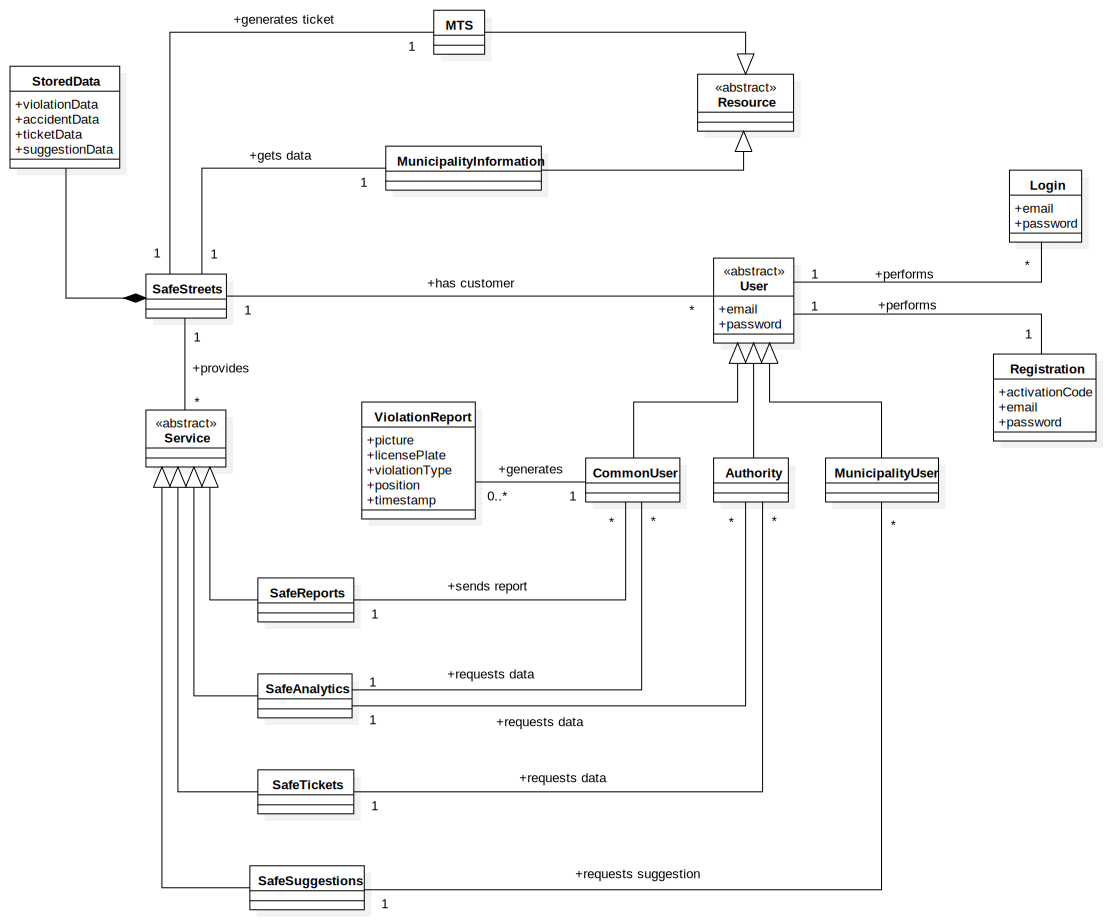
\includegraphics[width=\textwidth]{class_diagram}
\caption{Class diagram}
\end{figure}

As mentioned in the previous section, a service is exploited differently
depending on the type of user that is enjoying it. This is important
when considering SafeAnalytics, which has a crucial role in the
application, but is developed both to common users and authorities.
These types of users have different rights when accessing data stored by
SafeStreets, and will be provided with different query interfaces to
make their requests. If referring to the diagram, one could think to the
classes as the processes inherent to specific functionalities, and to
the relations as the interfaces provided to the users to enjoy a
service.\\
Relations between application and the resources do not need further
explanation, as they are deeply analyzed in the following sections to
describe how the interaction works.

\subsubsection{State diagrams}

In the diagrams shown below are emphasized the possible states of the
entities, and the transitions between one state to another.

\begin{figure}[H]
\centering
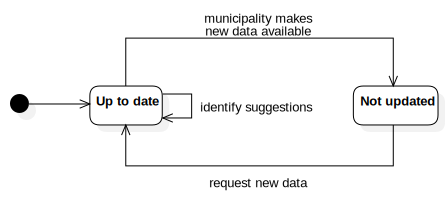
\includegraphics[width=\textwidth]{state_diagram_application}
\caption{Application}
\end{figure}

\begin{figure}[H]
\centering
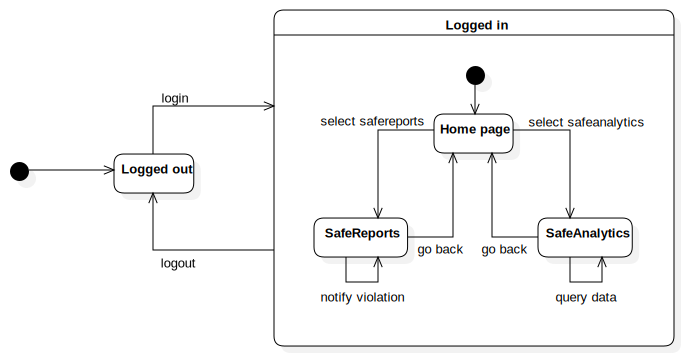
\includegraphics[width=\textwidth]{state_diagram_common_user}
\caption{Common user}
\end{figure}

\begin{figure}[H]
\centering
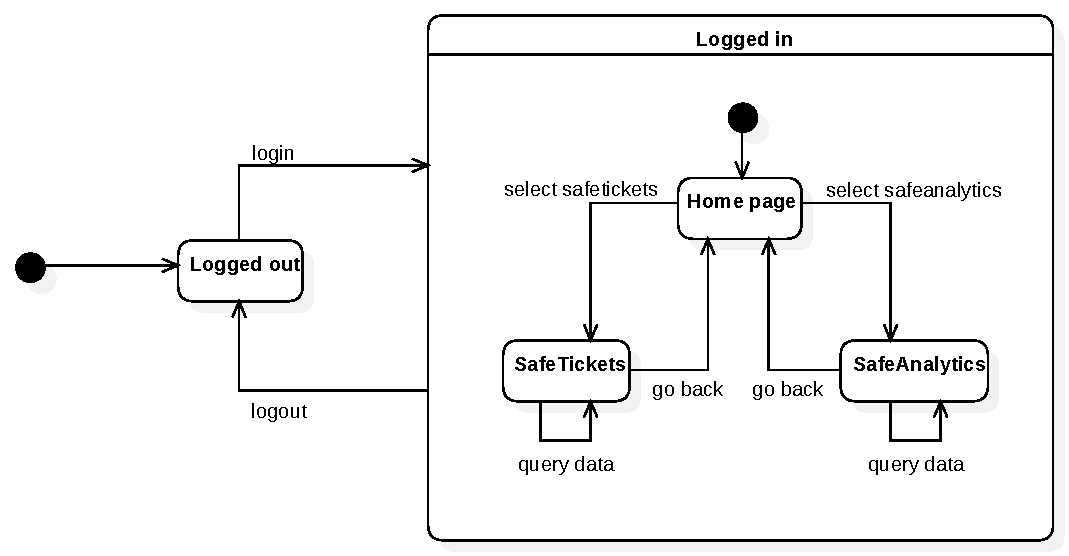
\includegraphics[width=\textwidth]{state_diagram_authority}
\caption{Authority}
\end{figure}

\begin{figure}[H]
\centering
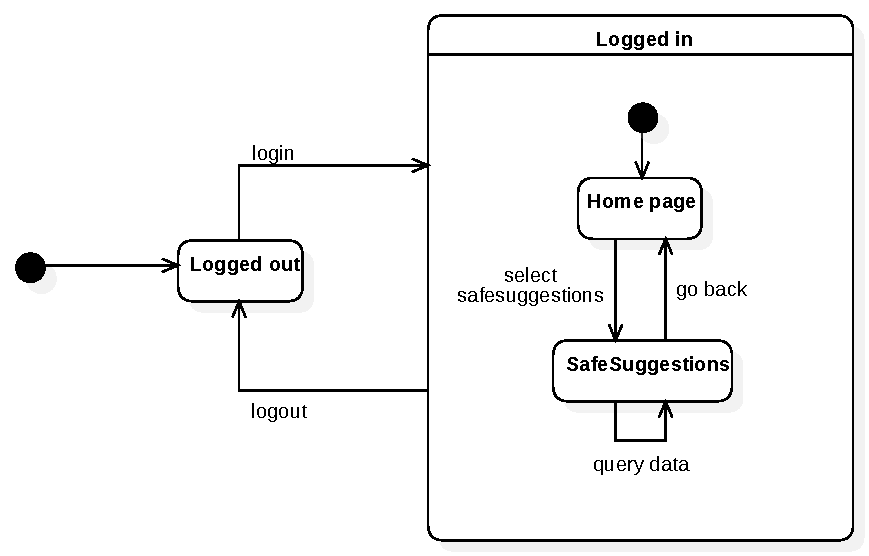
\includegraphics[width=\textwidth]{state_diagram_municipality_user}
\caption{Municipality user}
\end{figure}

\subsection{Product functions}

This section focuses on the definition of the functions to be provided
to reach the goals previously listed. For each service, a set of
requirements is identified. Later on in the document, these requirements
will be revised and factored to be mapped on the goals.

\subsubsection{SafeReports}

\begin{itemize}
\item
  The service must allow users to take pictures.
\item
  The service must forward pictures to OCR software to detect license
  plates.
\item
  The service must detect the timestamp.
\item
  The service must detect the position of the user.
\item
  The service must create a violation report filling it with the needed
  data.
\item
  The service must ask confirmation to the user before sending the
  violation report.
\item
  The service must check the integrity of the violation report before
  storing it.
\item
  The service must check for duplicated events before storing the
  violation report.
\item
  The service must forward stored violation report to MTS.
\item
  The service must store information on issued tickets when forwarding
  violation reports.
\end{itemize}

\subsubsection{SafeAnalytics}

\begin{itemize}
\item
  The service must provide users with a query interface.
\item
  The service must allow common users to select a time interval in the
  query interface.
\item
  The service must allow common users to select a day as a minimum
  granularity of the time interval.
\item
  The service must allow common users to select a zone in the query
  interface.
\item
  The service must allow common users to select 1 kilometer as the
  minimum granularity of the zone.
\item
  The service must allow common users to select a violation type in the
  query interface.
\item
  The service must allow authorities to access a special query
  interface.
\item
  The service must allow authorities to consult all the information
  stored.
\item
  The service must allow authorities to select a license plate in the
  special query interface.
\item
  The service must allow authorities to see the pictures of the
  violations.
\item
  The service must allow authorities to filter data using any
  granularity.
\end{itemize}

\subsubsection{SafeTickets}

\begin{itemize}
\item
  The service must provide authorities with a query interface.
\item
  The service must allow authorities to consult all the stored data
  about issued tickets.
\item
  The service must allow authorities to use the same filters of
  SafeAnalytics.
\item
  The service must allow going back to the violation report from which
  the tickets were generated.
\end{itemize}

\subsubsection{SafeSuggestions}

\begin{itemize}
\item
  The service must provide municipality users with a query interface.
\item
  The service must allow municipality users to request a suggestion
  using the query interface.
\item
  The service must allow municipality users to select a type of
  violation in the query interface.
\item
  The service must allow municipality users to select a zone in the
  query interface.
\item
  The service must provide suggestions to reduce the incidence of the
  selected violation in the selected zone.
\end{itemize}

\subsection{User characteristics}

As previously mentioned, several types of users can be identified. Every
type of user has different needs and limitations, that must be satisfied
providing different services. In this section, users are analyzed with
relation to their characteristics, to formally define these needs and
limitations.

\subsubsection{Common users}

Common users are the core of the application and the channel through
which the application collects data. Common users contribute to building
the data set that they can query to get data about violations. They must
be guided through the process of notification to make it easy and
intuitive and must be provided with the possibility to select the
correct filters to query the stored data.

\subsubsection{Authorities}

Authorities are, from a certain point of view, supervisors of the stored
data. They are not provided with the possibility to notify violations
(it is not what the authority account was designed for), but they can
access all the stored data about both notified violations and issued
tickets. For this type of account is not so important the easiness of
the interaction. Instead, it is very important to provide authorities
with the possibility to use powerful filters to query data.

\subsubsection{Municipality users}

The needs of the municipality users are somehow disjoint from those of
other users. This type of account is designed to give the possibility to
get the suggestions identified by the application. Because of this,
municipality users are not provided with the possibility to query the
stored data or to notify violations. Instead, they are provided with a
special query interface that allows them to select filters depending on
which type of intervention they want to put in place.

\subsection{Assumptions and dependencies}

\subsubsection{Domain assumptions}

\begin{itemize}
\item
  \textbf{D1} Users do not modify reality to generate fake violation
  reports.
\item
  \textbf{D2} The violations notified by the users are coherent with the
  taken pictures.
\item
  \textbf{D3} There exists a finite set of violations.
\item
  \textbf{D4} There exists a finite number of possible interventions.
\item
  \textbf{D5} Devices running SafeStreets has a working camera.
\item
  \textbf{D6} The camera is always safe (it is not possible to alter the
  data acquired by the camera).
\item
  \textbf{D7} Devices running SafeStreets are always able to get the
  timestamp.
\item
  \textbf{D8} Devices running SafeStreets are always able to detect the
  position with an error of at least 5 meters.
\item
  \textbf{D9} Internet connection is supposed to work whenever a user
  wants to use SafeStreets.
\item
  \textbf{D10} If OCR software returns a result, it is supposed to be
  correct.
\item
  \textbf{D11} If OCR software is not able to recognize a plate, it
  returns a special response.
\item
  \textbf{D12} A violation report is anonymous if and only if it
  consists only of the type of violation, position, and date.
\item
  \textbf{D13} Authorities and municipality users are previously
  verified.
\item
  \textbf{D14} Data from the municipality is reliable.
\end{itemize}

\subsubsection{Dependencies}

There are not strong dependencies between the services developed by the
application. There is a clear distinction between services that store
data and services that access data, thanks to this they can be exploited
independently one from each other. It is obvious that accessing the same
data set, it is useless to exploit services without storing data, so the
utility of the query services is bound to the existence of data
collection services.

\begin{itemize}
\item
  SafeAnalytics is based on data collection through SafeReports.
\item
  SafeTickets is based on the data collection from MTS.
\item
  SafeSuggestions is based on the data collection from the municipality
  data set.
\end{itemize}

Stronger dependencies exist between SafeStreets and the external
services to whom some tasks are delegated.

\begin{itemize}
\item
  SafeReports uses external OCR software.
\item
  SafeStreets is based on the GoogleMaps API.
\end{itemize}

The characteristic of these dependencies is that the link is not
exclusive with the service to which the tasks are delegated, in the
sense that services can be changed. OCR software can be any, and
OpenStreetMaps API can be used instead of GoogleMaps ones.

\newpage

\section{SPECIFIC REQUIREMENTS}\label{specific_requirements}

\subsection{External Interface Requirements}

\subsubsection{User Interfaces}

The following mockups are made to give an idea of how the user
interfaces should look like after the developing process. The mockups
represent the core services of SafeStreets focusing on the interaction
between the users and the system.
\bigskip\bigskip
\begin{figure}[H]
\centering
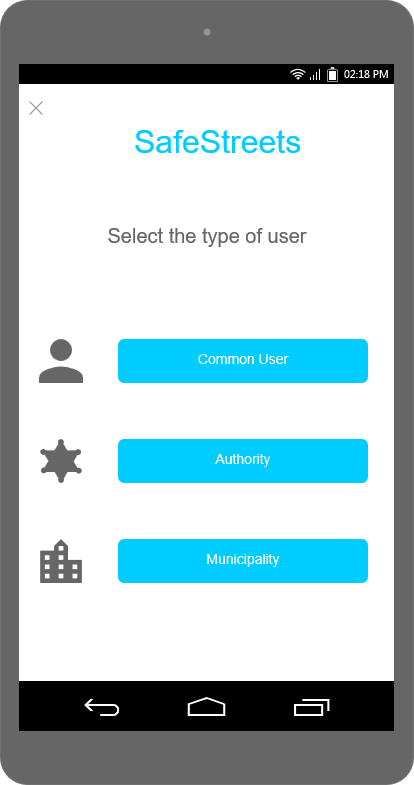
\includegraphics[height=\mockupheight]{mockup/choose_user}
\caption{The choice between different types of users.}
\end{figure}

\begin{figure}[H]
\centering
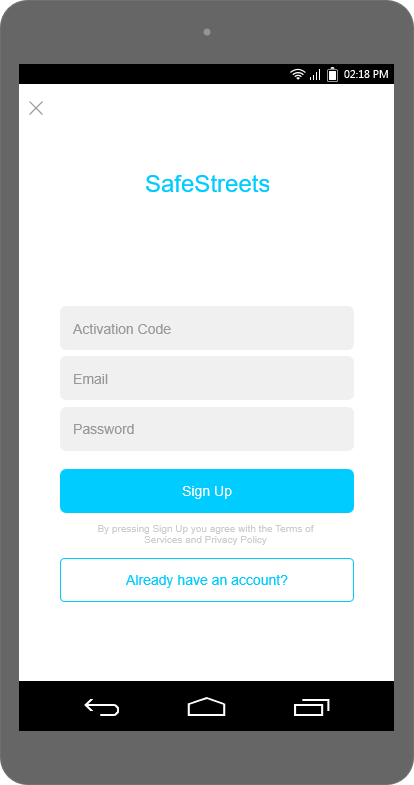
\includegraphics[height=\mockupheight]{mockup/sign_up}
\caption{The sign-up process for the municipality user.}
\end{figure}

\begin{figure}[H]
\centering
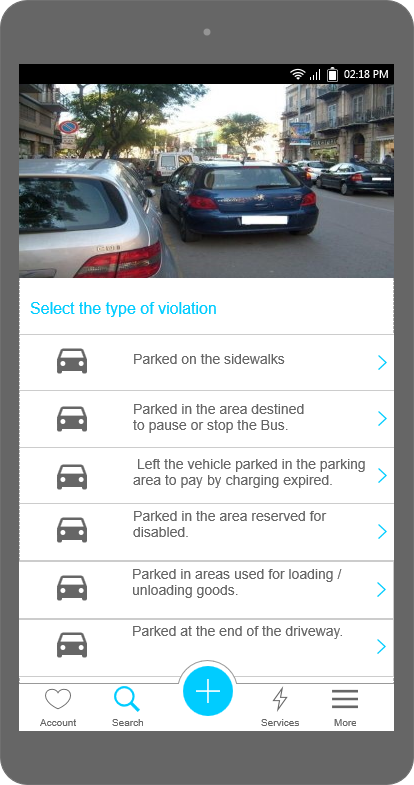
\includegraphics[height=\mockupheight]{mockup/select_violation}
\caption{Selection of the type of violation after a user took a
picture.}
\end{figure}

\begin{figure}[H]
\centering
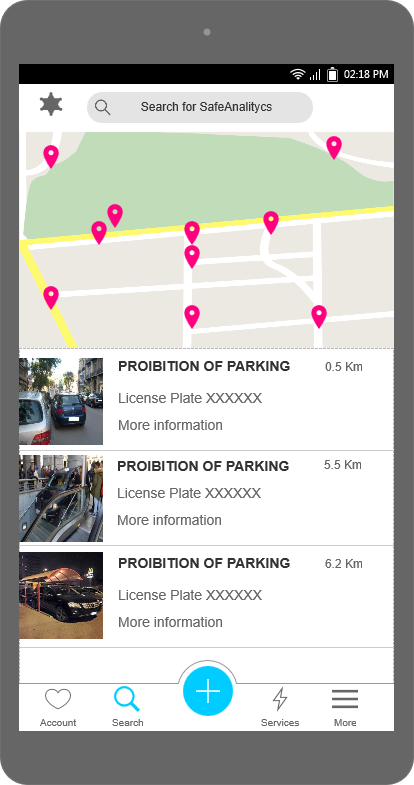
\includegraphics[height=\mockupheight]{mockup/get_violations}
\caption{The result of a query for violations made by an
authority. Authorities can see all the data stored and can click on a
specific violation for more information.}
\end{figure}

\begin{figure}[H]
\centering
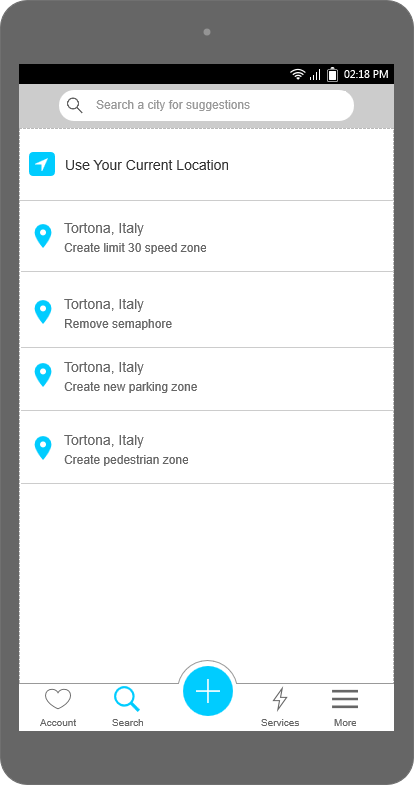
\includegraphics[height=\mockupheight]{mockup/get_suggestions}
\caption{The result of a query using SafeSuggestions. For more
information, the user needs to click on the selected suggestion.}
\end{figure}

\subsubsection{Hardware Interfaces}

The system does not provide any hardware interface.

\subsubsection{Software Interfaces}

The system does not provide any software interface.

\subsubsection{Communication Interfaces}

The system does not provide any communication interface.

\subsection{Functional Requirements}

\subsubsection{Scenarios}

\paragraph{Scenario 1}
Ted Mosby, a very honest architect, is tired of seeing cars parked in
the red zone right in front of his house. He told the problem to some
police agents in the past but nothing happened. He wants to report these
violations again but he doesn't know how to do it. Fortunately, Barney,
a public employee, suggests him to download and use the new SafeStreets
application for reporting violations. After signing up identifying
himself as a common user and inserting the email and password he can
finally report the violation. Mosby just needs to activate the GPS and
the internet connection and take a picture of the violation. He selects
the type of violation from a predefined list. After that, he is asked to
confirm the plate of the violating vehicle. He finally waits for the
outcome of his violation report.

\paragraph{Scenario 2}
Sheldon, a theoretical physicist, is currently studying the complexity
theory. He thinks that in big cities with a huge amount of traffic the
number of traffic violations is much larger than in small cities and
villages. Since Sheldon moved to Milan recently, he wants to know the
areas of Milan with the highest levels of traffic violations to avoid
parking in dangerous places. Sheldon knows about the SafeStreets app. He
logs in inserting his email and password and makes a query for all the
traffic violations reported in the last month in Milan. The results are
anonymized preserving the privacy of the violators and then sent back to
Sheldon. Sheldon can now park in safe areas.

\paragraph{Scenario 3}
Chuck, a policeman, was notified about a stolen car. He gets the idea of
looking for its possible traffic violations, to find it. He uses
SafeAnalytics to retrieve information about it, searching for its
license plate. Chuck discovers that the car is often parked on certain
reserved parking and finds the car in that location.

\paragraph{Scenario 4}
Seamus, the police chief, needs to collect the more money he can from
traffic tickets, to fund the construction of another police station.
Thanks to SafeTickets, he can identify the areas in which more traffic
tickets are generated and focus on those areas.

\paragraph{Scenario 5}
Giovanni, a municipality officer of the city of Milan, is looking for
possible interventions in the city, to improve the mobility of his area.
Giovanni logs in SafeStreets and accesses SafeSuggestions. He is
suggested to build a barrier near the sidewalk in Via Golgi, due to the
frequent parking violations that occur there.

\subsubsection{Common users}

\begin{figure}[H]
\centering
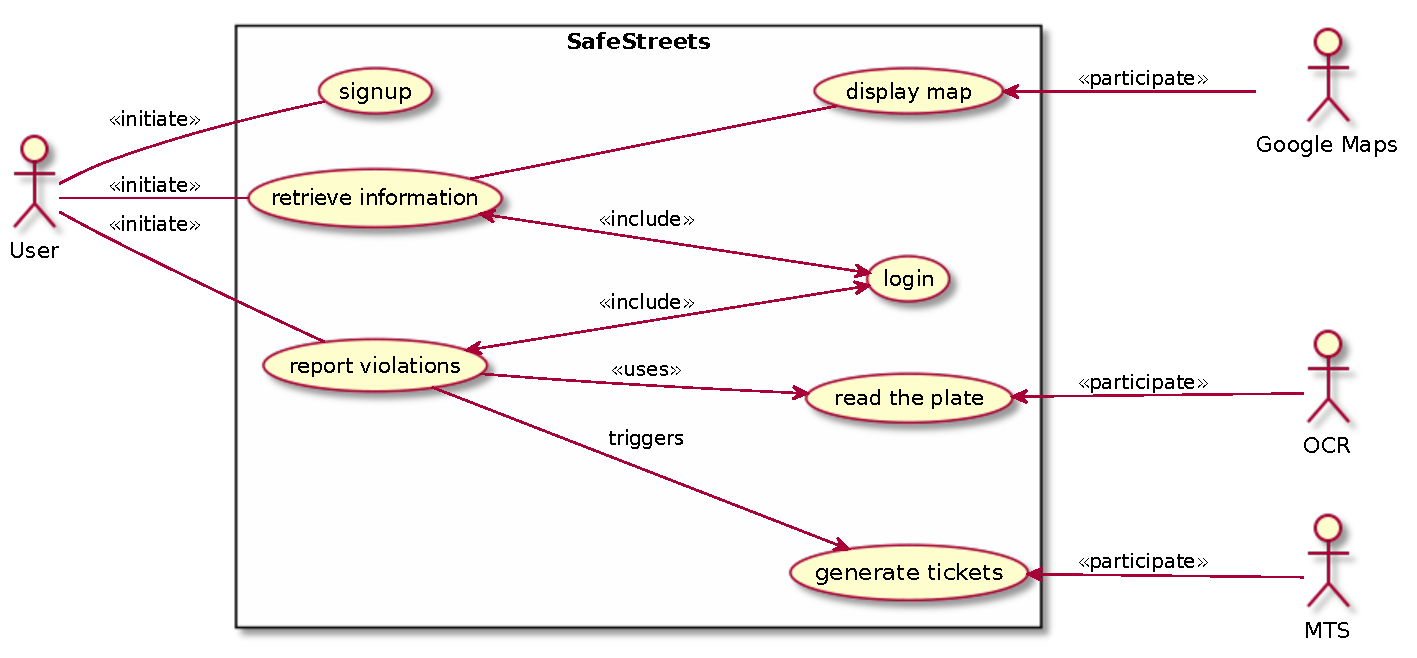
\includegraphics[width=\textwidth]{usecase_common_user.pdf}
\caption{Use cases diagram}
\end{figure}

\begin{table}[H]
\centering
\begin{tabularx}{\textwidth}{|l|X|}
\hline
Name & Sign up\tabularnewline
\hline
Actors &
\begin{itemize}[nosep,leftmargin=*]
\item Common user
\end{itemize}
\tabularnewline
\hline
Entry conditions &
\begin{itemize}[nosep,leftmargin=*]
\item The user opens the app on his smartphone
\end{itemize}
\tabularnewline
\hline
Events flow &
\begin{itemize}[nosep,leftmargin=*]
\item The user clicks on the sign up button
\item The user selects the option to identify himself as a common user
\item The user fills the forms with his email and a password
\item The system confirms his data
\item The system adds the new user to his data
\end{itemize}
\tabularnewline
\hline
Exit conditions &
\begin{itemize}[nosep,leftmargin=*]
\item The users is now registered and his account is registered to the
system
\end{itemize}
\tabularnewline
\hline
Exceptions &
\begin{itemize}[nosep,leftmargin=*]
\item The user has already an account. In this case the system suggests
the user to click the login button instead or to use another email
\end{itemize}
\tabularnewline
\hline
\end{tabularx}
\end{table}

\begin{table}[H]
\centering
\begin{tabularx}{\textwidth}{|l|X|}
\hline
Name & Login\tabularnewline
\hline
Actors &
\begin{itemize}[nosep,leftmargin=*]
\item Common user
\end{itemize}
\tabularnewline
\hline
Entry conditions &
\begin{itemize}[nosep,leftmargin=*]
\item The users opens the app on his device
\item The user has already signed up
\end{itemize}
\tabularnewline
\hline
Events flow &
\begin{itemize}[nosep,leftmargin=*]
\item The users presses the login button
\item The users types the email and the password
\item The system confirms the successful login
\end{itemize}
\tabularnewline
\hline
Exit conditions &
\begin{itemize}[nosep,leftmargin=*]
\item The user is logged in and is able to use the SafeStreets services
\end{itemize}
\tabularnewline
\hline
Exceptions &
\begin{itemize}[nosep,leftmargin=*]
\item The user types the wrong email or password. In both cases the system
sends an error to the user asking him to try the email password
combination again
\end{itemize}
\tabularnewline
\hline
\end{tabularx}
\end{table}

\begin{table}[H]
\centering
\begin{tabularx}{\textwidth}{|l|X|}
\hline
Name & Report a violation\tabularnewline
\hline
Actors &
\begin{itemize}[nosep,leftmargin=*]
\item Common user
\item OCR
\end{itemize}
\tabularnewline
\hline
Entry conditions &
\begin{itemize}[nosep,leftmargin=*]
\item The user has already done the login
\end{itemize}
\tabularnewline
\hline
Events flow &
\begin{itemize}[nosep,leftmargin=*]
\item The user takes a picture of the traffic violation
\item The required metadata are automatically added to the picture
\item The user selects the type of violation from a list of violations
\item The picture is sent to the OCR software to automatically scan and
read the plate
\item After receiving the plate from the OCR, the system asks the user to
confirm the plate of the violation vehicle
\item After the confirmation the system checks if the new violation is
equivalent to an already stored one
\item The system checks the integrity of the report
\item The systems stores the violation report if and only if the previous
equivalence check returned a negative result and the integrity test was
positive
\end{itemize}
\tabularnewline
\hline
Exit conditions &
\begin{itemize}[nosep,leftmargin=*]
\item The user receives a notification about the outcome of its violation
\end{itemize}
\tabularnewline
\hline
Exceptions &
\begin{itemize}[nosep,leftmargin=*]
\item If the OCR is not able to read the plate then the system sends an
error to the user and asks him to repeat the procedure
\end{itemize}
\tabularnewline
\hline
\end{tabularx}
\end{table}

\begin{table}[H]
\centering
\begin{tabularx}{\textwidth}{|l|X|}
\hline
Name & Generate tickets\tabularnewline
\hline
Actors &
\begin{itemize}[nosep,leftmargin=*]
\item SafeStreets
\item MTS
\end{itemize}
\tabularnewline
\hline
Entry conditions &
\begin{itemize}[nosep,leftmargin=*]
\item The system has validated and stored a new traffic violation report
\end{itemize}
\tabularnewline
\hline
Events flow &
\begin{itemize}[nosep,leftmargin=*]
\item The system forwards the violation report to MTS
\item MTS generates tickets from the violation report
\item MTS sends the results to SafeStreets
\end{itemize}
\tabularnewline
\hline
Exit conditions &
\begin{itemize}[nosep,leftmargin=*]
\item The system stores data about issued tickets and builds statistics
from that data
\end{itemize}
\tabularnewline
\hline
Exceptions &
\begin{itemize}[nosep,leftmargin=*]
\item If MTS is not able to generate the tickets then and error is sent to
SafeStreets and no data about issued tickets is stored
\end{itemize}
\tabularnewline
\hline
\end{tabularx}
\end{table}

\begin{table}[H]
\centering
\begin{tabularx}{\textwidth}{|l|X|}
\hline
Name & Retrieve information\tabularnewline
\hline
Actors &
\begin{itemize}[nosep,leftmargin=*]
\item Common user
\item Google Maps
\end{itemize}
\tabularnewline
\hline
Entry conditions &
\begin{itemize}[nosep,leftmargin=*]
\item The user has already done the login
\item The user wants to retrieve information about traffic violations
\end{itemize}
\tabularnewline
\hline
Events flow &
\begin{itemize}[nosep,leftmargin=*]
\item The user presses the button to start the query for the desired data
\item The user inserts the geographical filter for the query
\item The user inserts the time filter for the query
\item The system anonymizes the information
\item The results are sent to the user
\end{itemize}
\tabularnewline
\hline
Exit conditions &
\begin{itemize}[nosep,leftmargin=*]
\item The results are displayed in a map exploiting Google Maps' API
\end{itemize}
\tabularnewline
\hline
Exceptions & -\tabularnewline
\hline
\end{tabularx}
\end{table}

\begin{figure}[H]
\centering
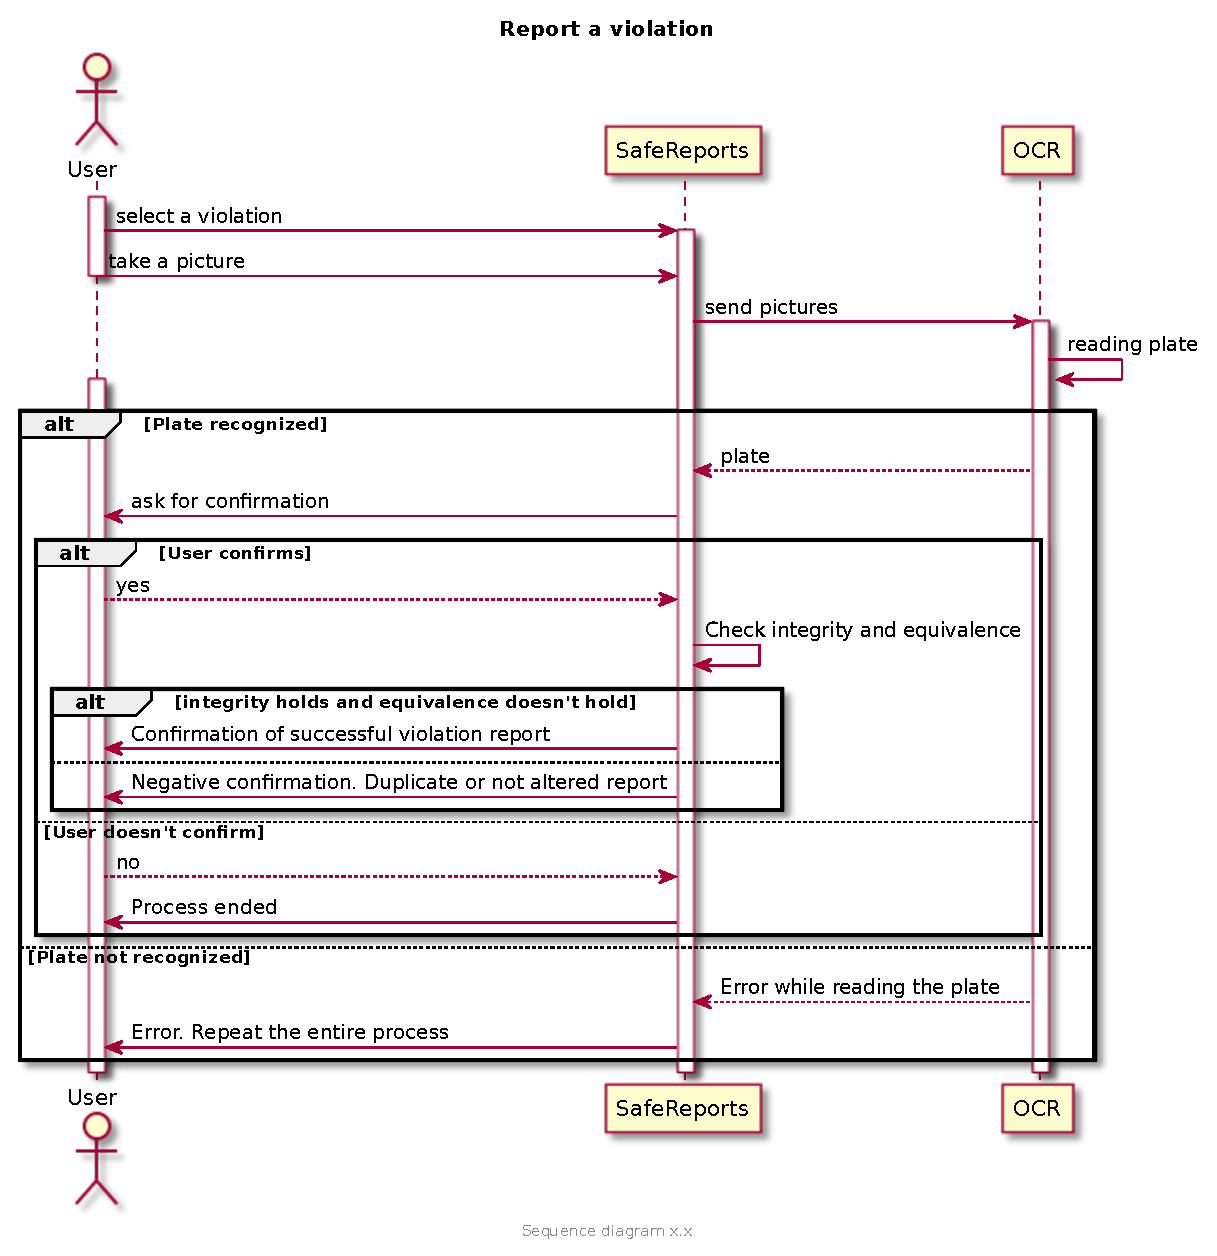
\includegraphics[width=\textwidth]{sequence_diagram_report}
\caption{Report a violation}
\end{figure}

\begin{figure}[H]
\centering
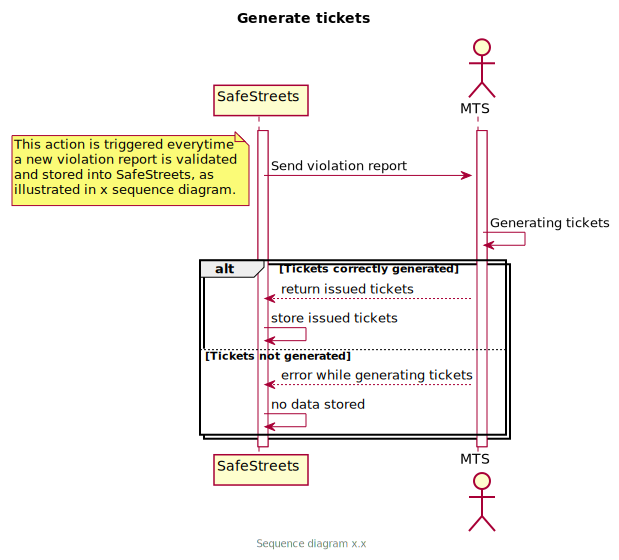
\includegraphics[width=0.85\textwidth]{sequence_tickets_generation}
\caption{Generate tickets}
\end{figure}

\begin{figure}[H]
\centering
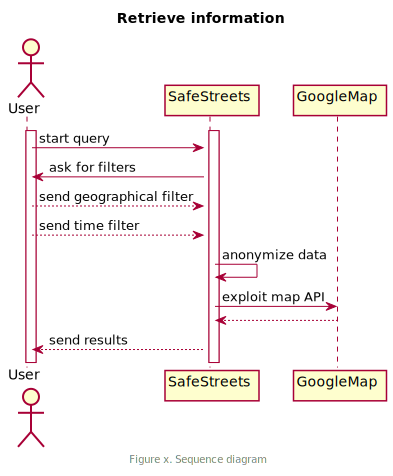
\includegraphics[width=0.55\textwidth]{sequence_diagram_retrieve_information}
\caption{Retrieve information}
\end{figure}

\subsubsection{Authorities}

\begin{figure}[H]
\centering
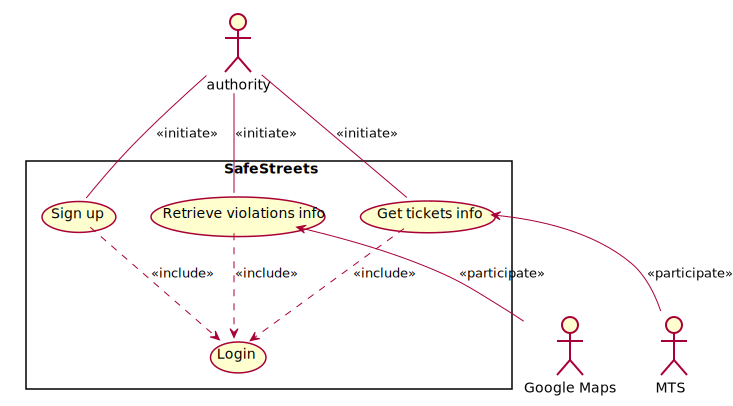
\includegraphics[width=\textwidth]{authorities_usecases}
\caption{Use cases diagram}
\end{figure}

\begin{table}[H]
\centering
\begin{tabularx}{\textwidth}{|l|X|}
\hline
Name & Sign up\tabularnewline
\hline
Actors &
\begin{itemize}[nosep,leftmargin=*]
\item Authority
\end{itemize}
\tabularnewline
\hline
Entry conditions &
\begin{itemize}[nosep,leftmargin=*]
\item The authority opens SafeStreets on his device
\end{itemize}
\tabularnewline
\hline
Events flow &
\begin{itemize}[nosep,leftmargin=*]
\item The authority chooses the sign up option
\item The authority selects the option to identify himself as authority
\item The authority inserts the activation code
\item The authority inserts his email and password
\item Authority confirms his data
\item SafeStreets saves his data
\end{itemize}
\tabularnewline
\hline
Exit conditions &
\begin{itemize}[nosep,leftmargin=*]
\item The authority is registered and his data are saved
\end{itemize}
\tabularnewline
\hline
Exceptions &
\begin{itemize}[nosep,leftmargin=*]
\item An account with the same email was already created. In this case
SafeStreets warns the authority and asks to change email or log in
\item The activation code is not valid. The authority is asked to reinsert
it
\item The authority doesn't provide all the data. In this case the system
asks him to insert them
\end{itemize}
\tabularnewline
\hline
\end{tabularx}
\end{table}

\begin{table}[H]
\centering
\begin{tabularx}{\textwidth}{|l|X|}
\hline
Name & Login\tabularnewline
\hline
Actors &
\begin{itemize}[nosep,leftmargin=*]
\item Authority
\end{itemize}
\tabularnewline
\hline
Entry conditions &
\begin{itemize}[nosep,leftmargin=*]
\item The authority has opened the application on his device
\item The authority is already registered
\end{itemize}
\tabularnewline
\hline
Events flow &
\begin{itemize}[nosep,leftmargin=*]
\item The authority chooses the login option
\item The authority inserts his email and password
\end{itemize}
\tabularnewline
\hline
Exit conditions &
\begin{itemize}[nosep,leftmargin=*]
\item The authority is identified
\end{itemize}
\tabularnewline
\hline
Exceptions &
\begin{itemize}[nosep,leftmargin=*]
\item The email is not registered. The authority is asked to reinsert it
or sign up
\item The password is incorrect. The authority is asked to reinsert it
\end{itemize}
\tabularnewline
\hline
\end{tabularx}
\end{table}

\begin{table}[H]
\centering
\begin{tabularx}{\textwidth}{|l|X|}
\hline
Name & Retrieve violation info\tabularnewline
\hline
Actors &
\begin{itemize}[nosep,leftmargin=*]
\item Authority
\item Google Maps
\end{itemize}
\tabularnewline
\hline
Entry conditions &
\begin{itemize}[nosep,leftmargin=*]
\item The authority is logged in SafeStreets
\item The authority wants to collect data about violations
\end{itemize}
\tabularnewline
\hline
Events flow &
\begin{itemize}[nosep,leftmargin=*]
\item The authority accesses the SafeAnalytics function
\item The authority selects the geographical filters
\item The authority selects the time filters
\item The authority selects the license plate filters
\item Data requested are sent to the authority
\end{itemize}
\tabularnewline
\hline
Exit conditions &
\begin{itemize}[nosep,leftmargin=*]
\item SafeStreets displays the data. If a map is required, it is provided
by Google Maps
\end{itemize}
\tabularnewline
\hline
Exceptions & -\tabularnewline
\hline
\end{tabularx}
\end{table}

\begin{table}[H]
\centering
\begin{tabularx}{\textwidth}{|l|X|}
\hline
Name & Get tickets info\tabularnewline
\hline
Actors &
\begin{itemize}[nosep,leftmargin=*]
\item Authority
\item MTS
\end{itemize}
\tabularnewline
\hline
Entry conditions &
\begin{itemize}[nosep,leftmargin=*]
\item The authority is logged in SafeStreets
\item The authority wants to get information about tickets issued by
SafeStreets
\end{itemize}
\tabularnewline
\hline
Events flow &
\begin{itemize}[nosep,leftmargin=*]
\item Authority accesses the SafeTickets functionality
\item The authority selects the geographical filters
\item The authority selects the time filters
\item The authority selects the license plate filters
\item Data requested are sent by SafeStreets to the authority
\end{itemize}
\tabularnewline
\hline
Exit conditions &
\begin{itemize}[nosep,leftmargin=*]
\item Safestreets displays the data
\end{itemize}
\tabularnewline
\hline
Exceptions & -\tabularnewline
\hline
\end{tabularx}
\end{table}

\begin{figure}[H]
\centering
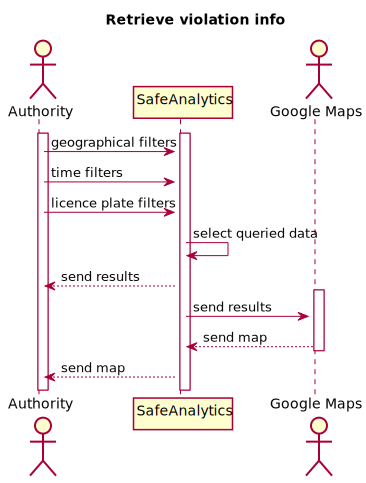
\includegraphics[width=0.65\textwidth]{retrieve_violation_info_sequence_diagram}
\caption{Retrieve violation info}
\end{figure}

\subsubsection{Municipality users}

\begin{figure}[H]
\centering
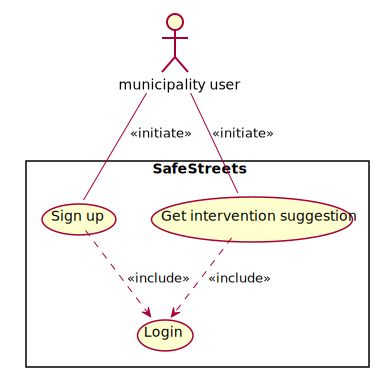
\includegraphics[width=\textwidth]{municipality_usecases}
\caption{Use cases diagram}
\end{figure}

\begin{table}[H]
\centering
\begin{tabularx}{\textwidth}{|l|X|}
\hline
Name & Get intervention suggestion\tabularnewline
\hline
Actors &
\begin{itemize}[nosep,leftmargin=*]
\item Municipality user
\end{itemize}
\tabularnewline
\hline
Entry conditions &
\begin{itemize}[nosep,leftmargin=*]
\item The municipality user has opened the application on his device and
logged in
\item The municipality user wants to get suggestions about possible
improvements
\end{itemize}
\tabularnewline
\hline
Events flow &
\begin{itemize}[nosep,leftmargin=*]
\item The municipality user accesses the SafeSuggestions functionality
\item The municipality user selects the geographical filters
\item SafeSuggestions gets possible interventions based on the filters
provided
\item SafeStreets sends (if available) the suggestion relative to the
filters provided
\end{itemize}
\tabularnewline
\hline
Exit conditions &
\begin{itemize}[nosep,leftmargin=*]
\item SafeStreets displays the suggestion (if given) or a "no suggestions"
notice
\end{itemize}
\tabularnewline
\hline
Exceptions & -\tabularnewline
\hline
\end{tabularx}
\end{table}

\begin{table}[H]
\centering
\begin{tabularx}{\textwidth}{|l|X|}
\hline
Name & Get accidents suggestion\tabularnewline
\hline
Actors &
\begin{itemize}[nosep,leftmargin=*]
\item Municipality
\end{itemize}
\tabularnewline
\hline
Entry conditions &
\begin{itemize}[nosep,leftmargin=*]
\item Timeout trigger is activated
\end{itemize}
\tabularnewline
\hline
Events flow &
\begin{itemize}[nosep,leftmargin=*]
\item New data is requested by SafeStreets from the municipality
\item The municipality evaluates if updates in data occurred
\item The municipality provides the new data to SafeStreets
\item Safestreets updates its data and builds new statistics in order to
generate new suggestions
\end{itemize}
\tabularnewline
\hline
Exit conditions &
\begin{itemize}[nosep,leftmargin=*]
\item The new suggestions are stored in the system
\end{itemize}
\tabularnewline
\hline
Exceptions & -\tabularnewline
\hline
\end{tabularx}
\end{table}

The use cases "Sign up" and "Login" are equal to the ones of the
authorities, and are omitted to avoid redundancies.

\begin{figure}[H]
\centering
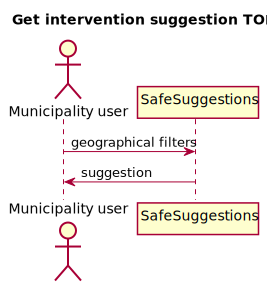
\includegraphics[width=0.7\textwidth]{get_intervention_suggestion_sequence_diagram}
\caption{Get intervention suggestion}
\end{figure}

\begin{figure}[H]
\centering
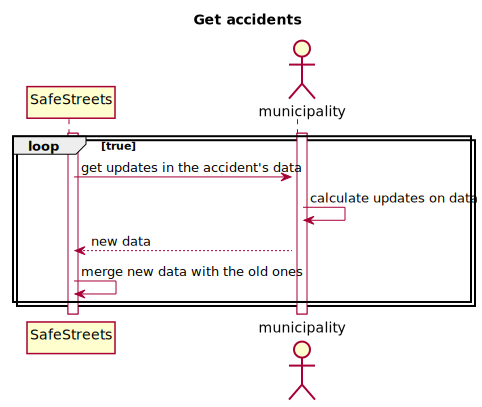
\includegraphics[width=0.9\textwidth]{get_accidents_sequence_diagram}
\caption{Get accidents}
\end{figure}

\subsubsection{Activities}

\begin{figure}[H]
\centering
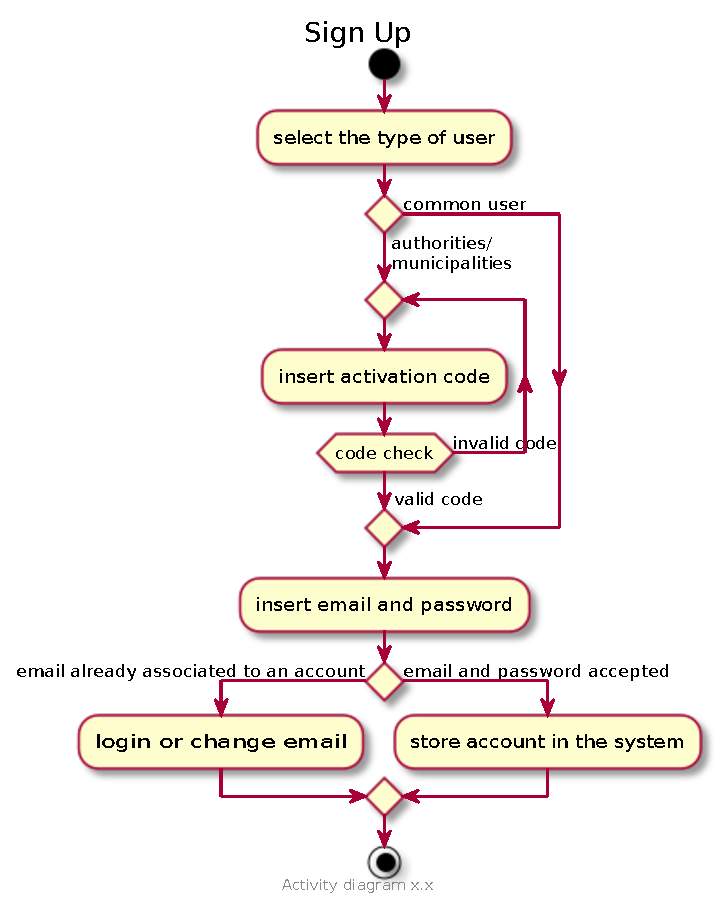
\includegraphics[width=\textwidth]{activity_diagram_login}
\caption{Registration}
\end{figure}

\begin{figure}[H]
\centering
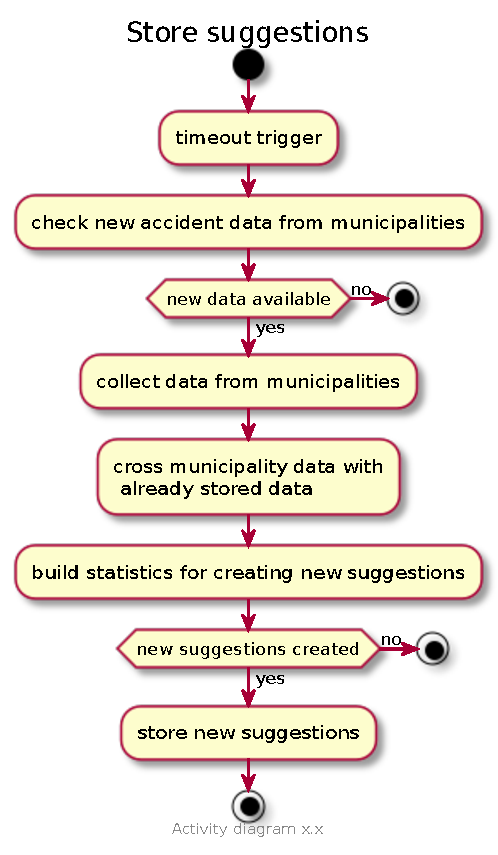
\includegraphics[width=0.7\textwidth]{activity_diagram_create_suggestions}
\caption{Generation of new suggestions}
\end{figure}

\subsubsection{Requirements}\label{header-n643}

\textbf{G1) SafeReports must allow common users to send violation
reports.}

\begin{itemize}
\item
  \textbf{R1} When a picture is taken using SafeReports, a new violation
  record is generated.
\item
  \textbf{R2} When a new violation record is generated, the current
  position of the user is added to the report.
\item
  \textbf{R3} When a new violation record is generated, the timestamp is
  added to the report.
\item
  \textbf{R4} When a new violation record is generated, the photo is
  scanned by an OCR software to automatically detect the plate.
\item
  \textbf{R5} If the OCR software fails in detecting the plate, the user
  is notified and asked to repeat the procedure.
\item
  \textbf{R6} If the OCR software detects the plate, the user is asked
  to confirm the violation report.
\item
  \textbf{R7} If the user confirms the violation report, it is sent to
  SafeStreets.
\item
  \textbf{R8} SafeStreets stores the information about the violation
  only if there aren't equivalent events already stored.
\end{itemize}

\textbf{G2) SafeAnalytics must allow common users to get anonymous data
on violations.}

\begin{itemize}
\item
  \textbf{R9} SafeAnalytics allows common users to get data about
  violations selecting zone, time and type of violation.
\item
  \textbf{R10} SafeAnalytics anonymizes information before sending it to
  common users.
\end{itemize}

\textbf{G3) SafeAnalytics must allow authorities to access to all the
data without restrictions.}

\begin{itemize}
\item
  \textbf{R11} SafeAnalytics allows authorities to get all the information
  stored by SafeStreets.
\end{itemize}

\textbf{G4) SafeSuggestions must allow municipality users to get
suggestions on possible interventions.}

\begin{itemize}
\item
  \textbf{R12} SafeStreets must store data about accidents provided by
  the municipality when available.
\item
  \textbf{R13} SafeStreets must analyze collected data crossed with data
  from the municipality to identify possible interventions.
\item
  \textbf{R14} SafeSuggestions allows municipality users to get
  suggestions provided by SafeStreets.
\end{itemize}

\textbf{G5) SafeStreets must generate traffic tickets forwarding
reliable data to MTS.}

\begin{itemize}
\item
  \textbf{R15} When the users send a violation report, its integrity is
  checked.
\item
  \textbf{R16} If the integrity check is not successful, the violation
  report is discarded.
\item
  \textbf{R17} SafeStreets must forward every new stored violation
  report to MTS to generate traffic tickets.
\end{itemize}

\textbf{G6) SafeTickets must allow authorities to get statistics on
issued tickets.}

\begin{itemize}
\item
  \textbf{R18} When a new ticket is generated using MTS, ticket-related
  data are stored by SafeStreets.
\item
  \textbf{R19} SafeStreets must build statistics from stored data about
  issued tickets.
\item
  \textbf{R20} SafeTickets allows authorities to get information and
  statistics on issued tickets.
\end{itemize}

\subsubsection{Traceability matrix}\label{header-n696}

\begin{table}[H]
\centering
\begin{tabular}{|l|l|l|}
\hline
Requirements & Goal & Use case\tabularnewline
\hline
R1 & G1 & Report violations\tabularnewline
R2 & G1 & Report violations\tabularnewline
R3 & G1 & Report violations\tabularnewline
R4 & G1 & Report violations\tabularnewline
R5 & G1 & Report violations\tabularnewline
R6 & G1 & Report violations\tabularnewline
R7 & G1 & Report violations\tabularnewline
R8 & G1 & Report violations\tabularnewline
R9 & G2 & Retrieve information\tabularnewline
R10 & G2 & Retrieve information\tabularnewline
R11 & G3 & Retrieve violations info\tabularnewline
R12 & G4 & Get accidents\tabularnewline
R13 & G4 & Get accidents\tabularnewline
R14 & G4 & Get intervention suggestion\tabularnewline
R15 & G5 & Generate tickets\tabularnewline
R16 & G5 & Generate tickets\tabularnewline
R17 & G5 & Generate tickets\tabularnewline
R18 & G6 & Generate tickets\tabularnewline
R19 & G6 & Generate tickets\tabularnewline
R20 & G6 & Get tickets info\tabularnewline
\hline
\end{tabular}
\end{table}

\subsection{Performance Requirements}

\begin{itemize}
\item
  The system must be able to serve a great number of users reporting a
  violation simultaneously.
\item
  SafeAnalytics must be able to provide the data requested by both
  common users and authorities in less than 3 seconds, to provide the
  best experience.
\item
  The data about accidents provided by the municipality must be checked
  for updates at least every 5 minutes, to provide reliable and always
  updated suggestions.
\end{itemize}

\subsection{Design Constraints}

\subsubsection{Standards compliance}

The timestamp must adopt the ISO 8601 standard. The chain of custody of
the information coming from the user must never be broken, so the
correspondence of the data provided by a common user and the one
received by MTS must be guaranteed.

\subsubsection{Hardware limitations}

To correctly run the application, the device must have a camera with a
resolution sufficient to provide an understandable image, a working
internet connection, and a GPS.

\subsubsection{Any other constraint}

The system must not provide sensitive data to common users, so the
license plate and the photo of a violation must not be provided to them.

\subsection{Software System Attributes}

\subsubsection{Reliability}

SafeStreets must be fault-tolerant, so data must not be lost. This can
be achieved by keeping multiple copies of the data.

\subsubsection{Availability}

SafeStreets must be working 24/7.\\
SafeReports is expected to work with an availability of 99.999\%, as it
is the core of the application. The other functionalities can be
slightly less fault-tolerant, and be available 99.99\% of the time.

\subsubsection{Security}

The data provided by common users contain sensitive information, so
security is a crucial point. The databases on which data is collected
must be protected to avoid attacks, and the software must be GDPR
compliant. Data must be encrypted when sent, and the reliability of the
data received by MTS must be checked.

\subsubsection{Maintainability}

The code must be easy to fix and modify, to reduce the effort and the
cost of the modifications. It must avoid fast obsolescence, so be always
as aligned as possible to the new stable technologies.\\
The modularity of the code and the reusability of the logic (which needs
to be as separated as possible from the implementation) are needed to
guarantee the ease of maintenance in the future.

\subsubsection{Portability}

The software is thought to run on the majority of mobile devices, so it
should be developed for Android and iOS smartphones.

\newpage

\section{FORMAL ANALYSIS USING ALLOY}\label{formal_analysis_using_alloy}

\lstinputlisting[language=alloy]{resources/alloy/model.als}

\newpage

\lstinputlisting[language=alloy]{resources/alloy/world_no_confirmation.als}

\begin{figure}[H]
\centering
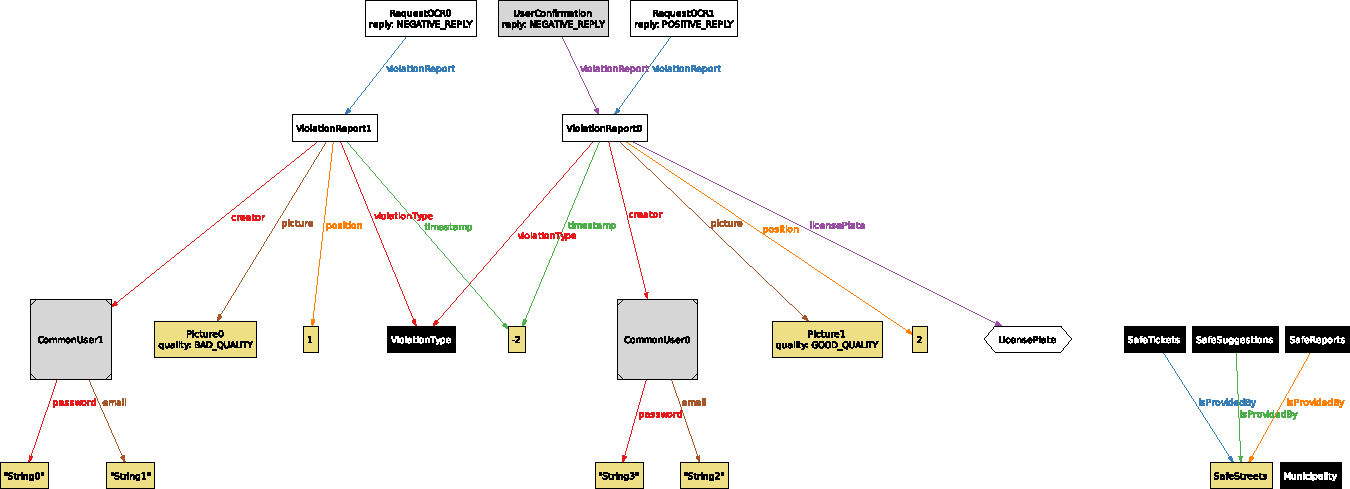
\includegraphics[width=\textwidth]{alloy/world_no_confirmation}
\caption{This world proves the consistency of the model when the violation
report is refused by the user and by the OCR software.}
\end{figure}

\newpage

\lstinputlisting[language=alloy]{resources/alloy/world_tickets_and_suggestions.als}

\begin{figure}[H]
\centering
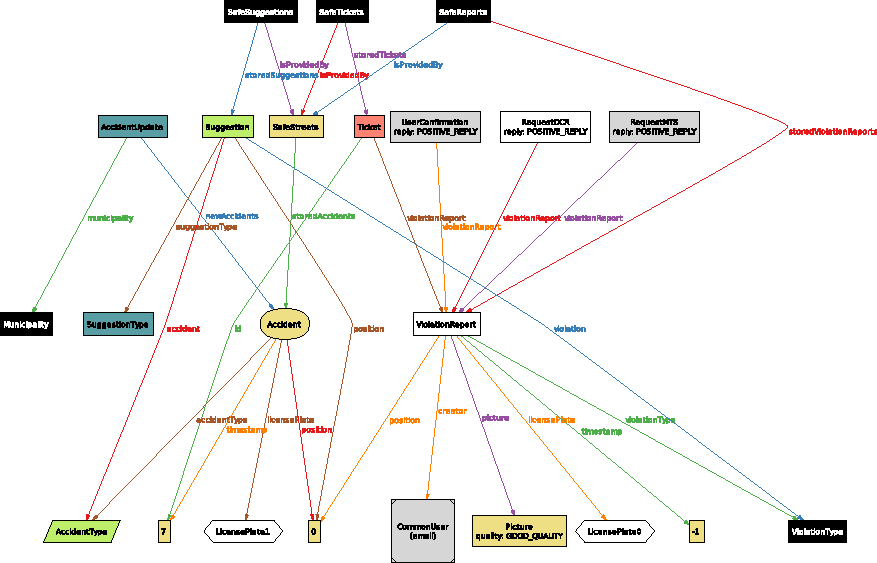
\includegraphics[width=\textwidth]{alloy/world_tickets_and_suggestions}
\caption{This world proves the consistency of the model when a violation
report is stored and a traffic ticket is generated.}
\end{figure}

\newpage

\lstinputlisting[language=alloy]{resources/alloy/world_accepted_violation.als}

\begin{figure}[H]
\centering
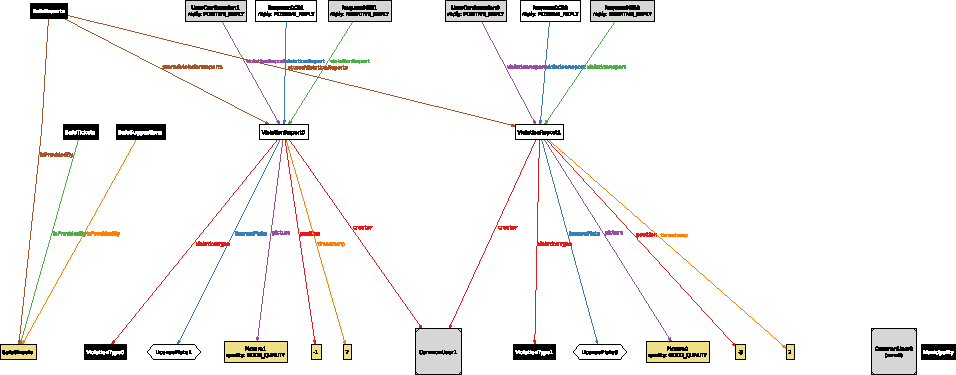
\includegraphics[width=\textwidth]{alloy/world_accepted_violation}
\caption{This world proves the consistency of the model when two violation
reports are stored, and no traffic ticket is generated.}
\end{figure}

\newpage

\lstinputlisting[language=alloy]{resources/alloy/world_report_query.als}

\begin{figure}[H]
\centering
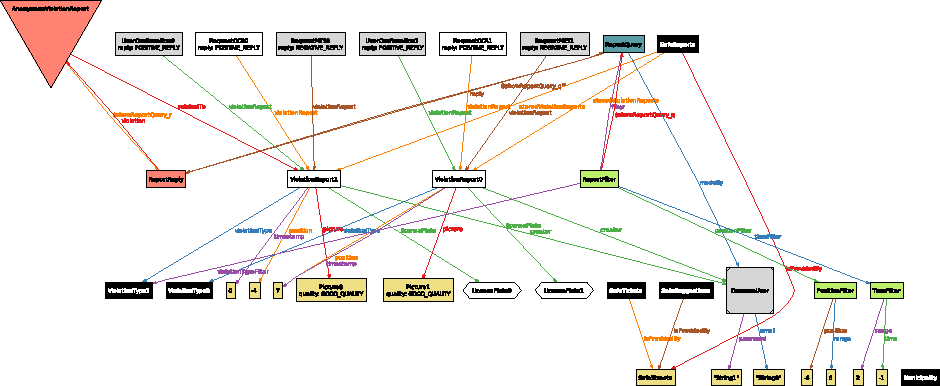
\includegraphics[width=\textwidth]{alloy/world_report_query}
\caption{This world proves the consistency of the model when a common user
makes a query on stored data.}
\end{figure}

\newpage

\lstinputlisting[language=alloy]{resources/alloy/world_super_report_query.als}

\begin{figure}[H]
\centering
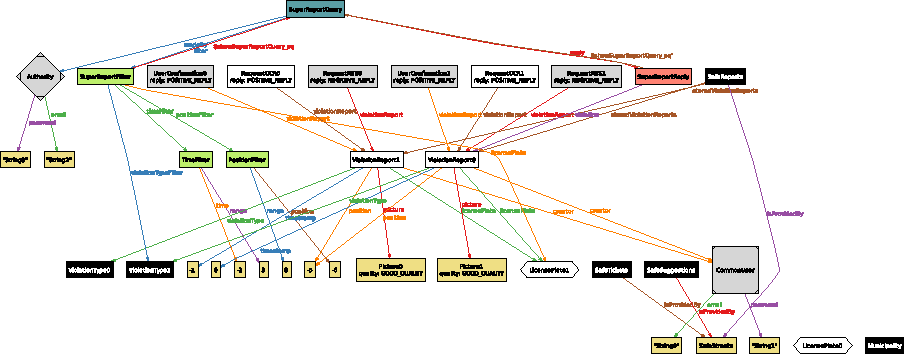
\includegraphics[width=\textwidth]{alloy/world_super_report_query}
\caption{This world proves the consistency of the model when an authority
makes a query on stored data.}
\end{figure}

\newpage

\lstinputlisting[language=alloy]{resources/alloy/world_ticket_query.als}

\begin{figure}[H]
\centering
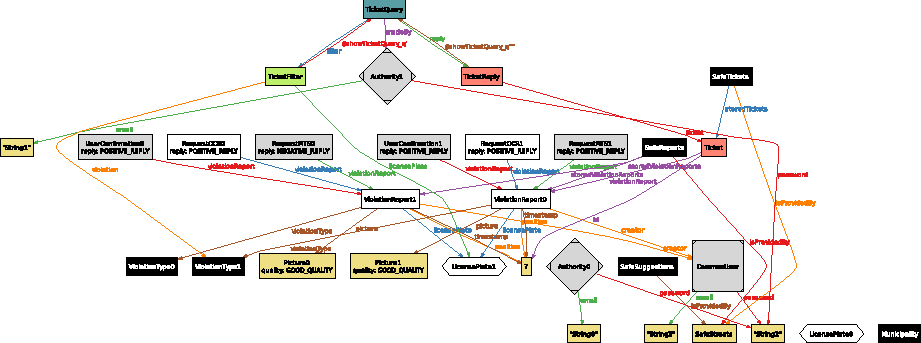
\includegraphics[width=\textwidth]{alloy/world_ticket_query}
\caption{This world proves the consistency of the model when an authority
makes a query on data about issued tickets.}
\end{figure}

\newpage

\lstinputlisting[language=alloy]{resources/alloy/world_suggestion_query.als}

\begin{figure}[H]
\centering
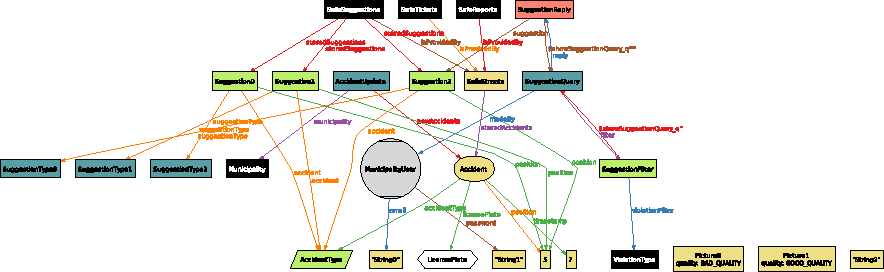
\includegraphics[width=\textwidth]{alloy/world_suggestion_query}
\caption{This world proves the consistency of the model when a
municipality user makes a query to get suggestions.}
\end{figure}

\newpage

\section{EFFORT SPENT}\label{effort_spent}

\begin{table}[H]
\centering
\begin{tabular}{|l|c|c|c|}
\hline
Task & Braga & Calderon & Favaro\tabularnewline
\hline
Introduction & 11 & 11 & 11\tabularnewline
Product perspective & 3 & 3 & 3\tabularnewline
Product functions & 2 & 2 & 2\tabularnewline
User characteristics & 2 & 2 & 2\tabularnewline
Assumptions and dependencies & 4 & 4 & 4\tabularnewline
External Interface Requirements & 3 & 3 & 3\tabularnewline
Functional Requirements & 12 & 12 & 12\tabularnewline
Performance Requirements & 1 & 1 & 1\tabularnewline
Design Constraints & 1 & 1 & 1\tabularnewline
Software System Attributes & 1 & 1 & 1\tabularnewline
Formal Analysis using Alloy & 17 & 17 & 17\tabularnewline
\hline
\end{tabular}
\end{table}

\section{REFERENCES}\label{references}

\begin{itemize}
\item
  Specification document "Mandatory Project Assignment" 2019-2020
\item
  IEEE Std 830-­1998 IEEE Recommended Practice for Software Requirements
  Specifications
\item
  UML diagrams:\\
  \url{https://www.uml-diagrams.org/}
\item
  Alloy:\\
  \url{http://alloytools.org/}
\end{itemize}

\end{document}